\section{Übersicht}

\begin{frame}
  {Übersicht}
  \onslide<+->
  \begin{itemize}[<+->]
    \item Übersicht über die wichtigen \alert{Schreibprinzipien}
      \Zeile
    \item \alert{Spatien} | Trennung syntaktischer Wörter
      \Zeile
    \item \alert{Positionsunabhängige Großschreibung}
      \Zeile
    \item Univerbierung von N und V
      \Zeile
    \item \citet{Schaefer2018b}
  \end{itemize}
\end{frame}



\section[Prinzipien]{Schreibprinzipien}

\begin{frame}
  {Zusammenfassung der besprochenen Schreibprinzipien I}
  \pause
  Korrespondenzen zur Phonologie\\
  \Zeile
  \pause
  \begin{itemize}[<+->]
    \item \alert{phonologisches Schreibprinzip}
      \begin{itemize}[<+->]
        \item Konsonantenzeichen (inkl.\ Di- und Trigraphen)\\
          entsprechen 1:1 zugrundeliegenden Segmenten.
        \item Paare von zugrundeliegendem gespanntem und ungespanntem Vokal\\
          entsprechen jeweils nur einem Vokalzeichen 
      \end{itemize}
     \Zeile 
    \item \alert{Prinzip der Silbengelenkschreibung}
      \begin{itemize}[<+->]
        \item Silbengelenke werden durch Konsonantendopplung markiert.
        \item Für Di- und Trigraphen gilt dies nicht.
      \end{itemize}
  \end{itemize}
\end{frame}

\begin{frame}
  {Zusammenfassung der besprochenen Schreibprinzipien II}
  Korrespondenzen zur Morphosyntax\\
  \Zeile
  \pause
  \begin{itemize}[<+->]
    \item \alert{Prinzip der Konstantschreibung}
      \begin{itemize}[<+->]
        \item Die Formen eines lexikalischen Wortes werden so ähnlich geschrieben,\\
          wie es angesichts der anderen Prinzipien möglich ist.
      \end{itemize}
      \Zeile
    \item \grau{Prinzip der Spatienschreibung}
      \begin{itemize}[<+->]
        \item \grau{Syntaktische Wörter werden durch Spatium getrennt.}
        \item \grau{Zweifelsfälle dabei sind morphosyntaktisch, nicht graphematisch.}
      \end{itemize}
      \Zeile
    \item \grau{Prinzip der positionsunabhängige Majuskelschreibung}
      \begin{itemize}[<+->]
        \item \grau{Substantive werden positionsunabhängig\\
        mit einleitender Majuskel geschrieben.}
      \end{itemize}
  \end{itemize}
\end{frame}



\section{Wörter -- Spatien}

\begin{frame}
  {Boustrophedon: Gesetze von Gortys}
  \pause
  \centering
  \includegraphics[width=0.8\textwidth]{\GRAPHPATH/gortys}\\
  {\tiny (Kreta; griechisch (dorisch), 6.--5.\ Jh.\ u.\,Zr.)}
\end{frame}

\begin{frame}
  {Scriptio continua: Genji no Monogatari}
  \pause
  \centering
  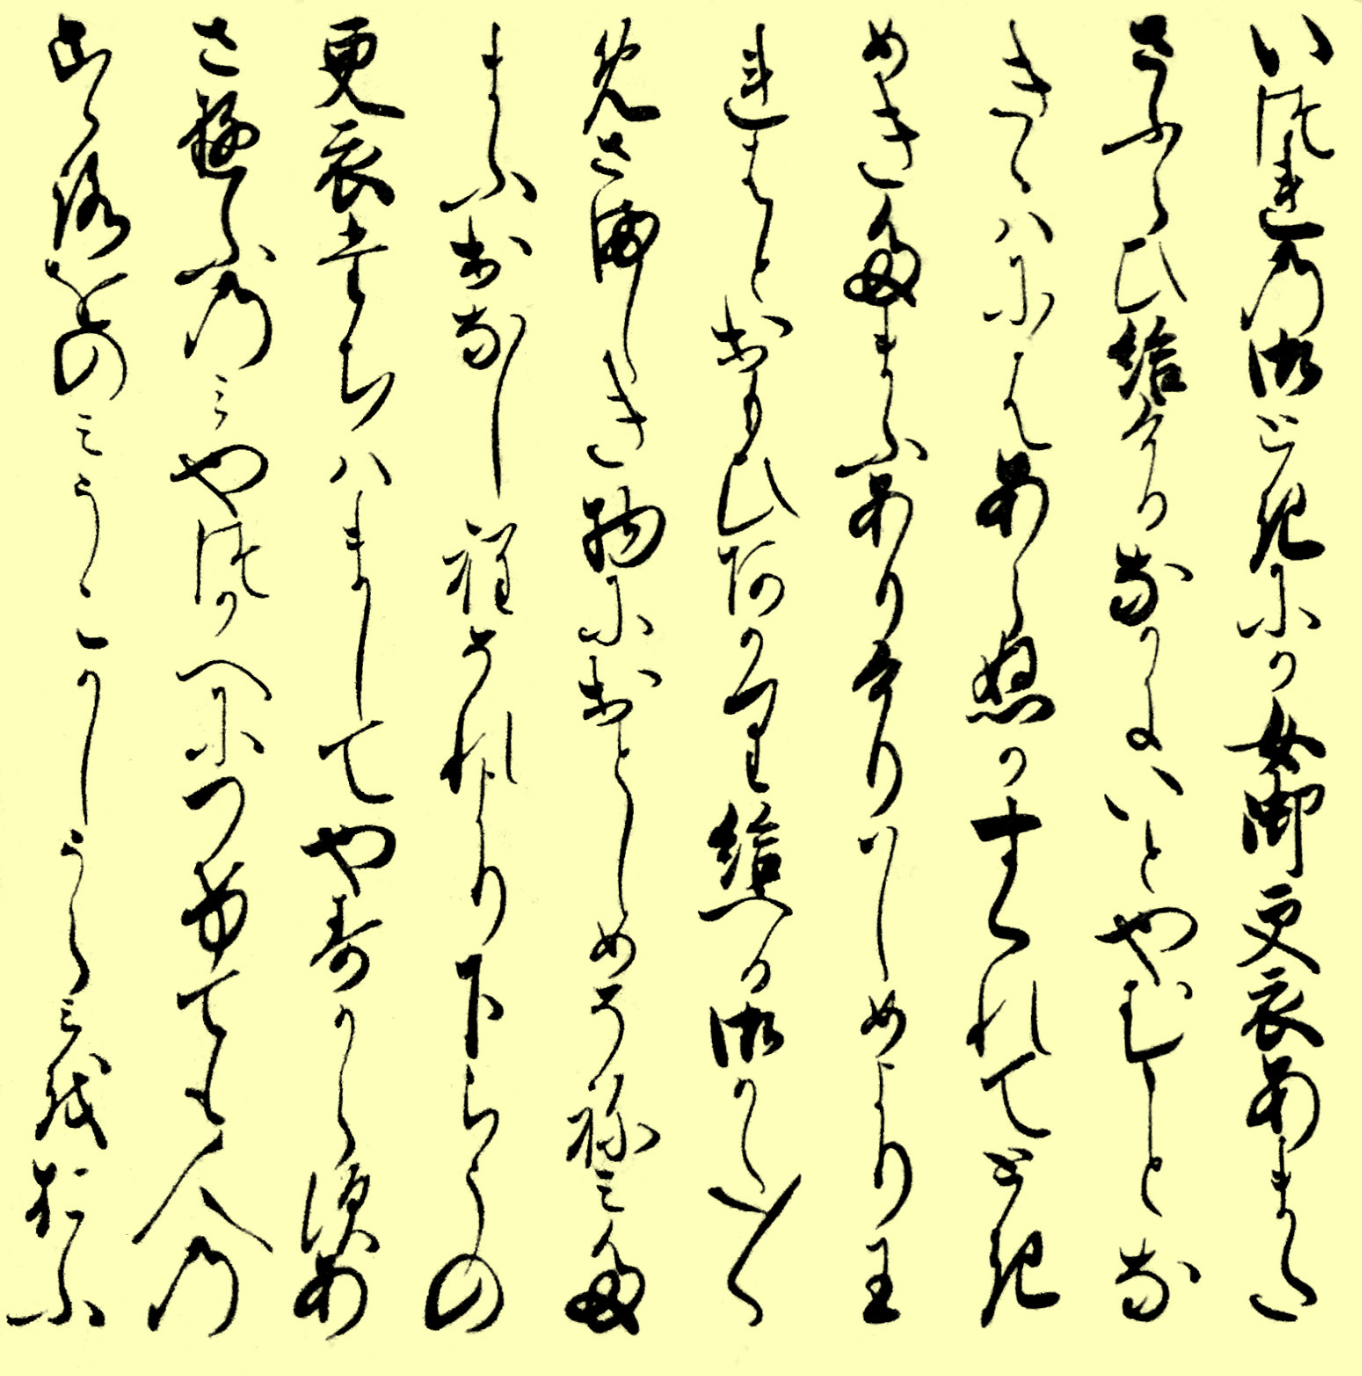
\includegraphics[width=0.55\textwidth]{\GRAPHPATH/genji1}\\
  {\tiny (\citealt{Rickmeyer1991}; 源氏物語:きりつぼ, ca. 1000 u.\,Zr., Manuskript ca.\ 1200 u.\,Zr.}
\end{frame}

\begin{frame}
  {Scriptio continua: Genji no Monogatari}
  \centering
  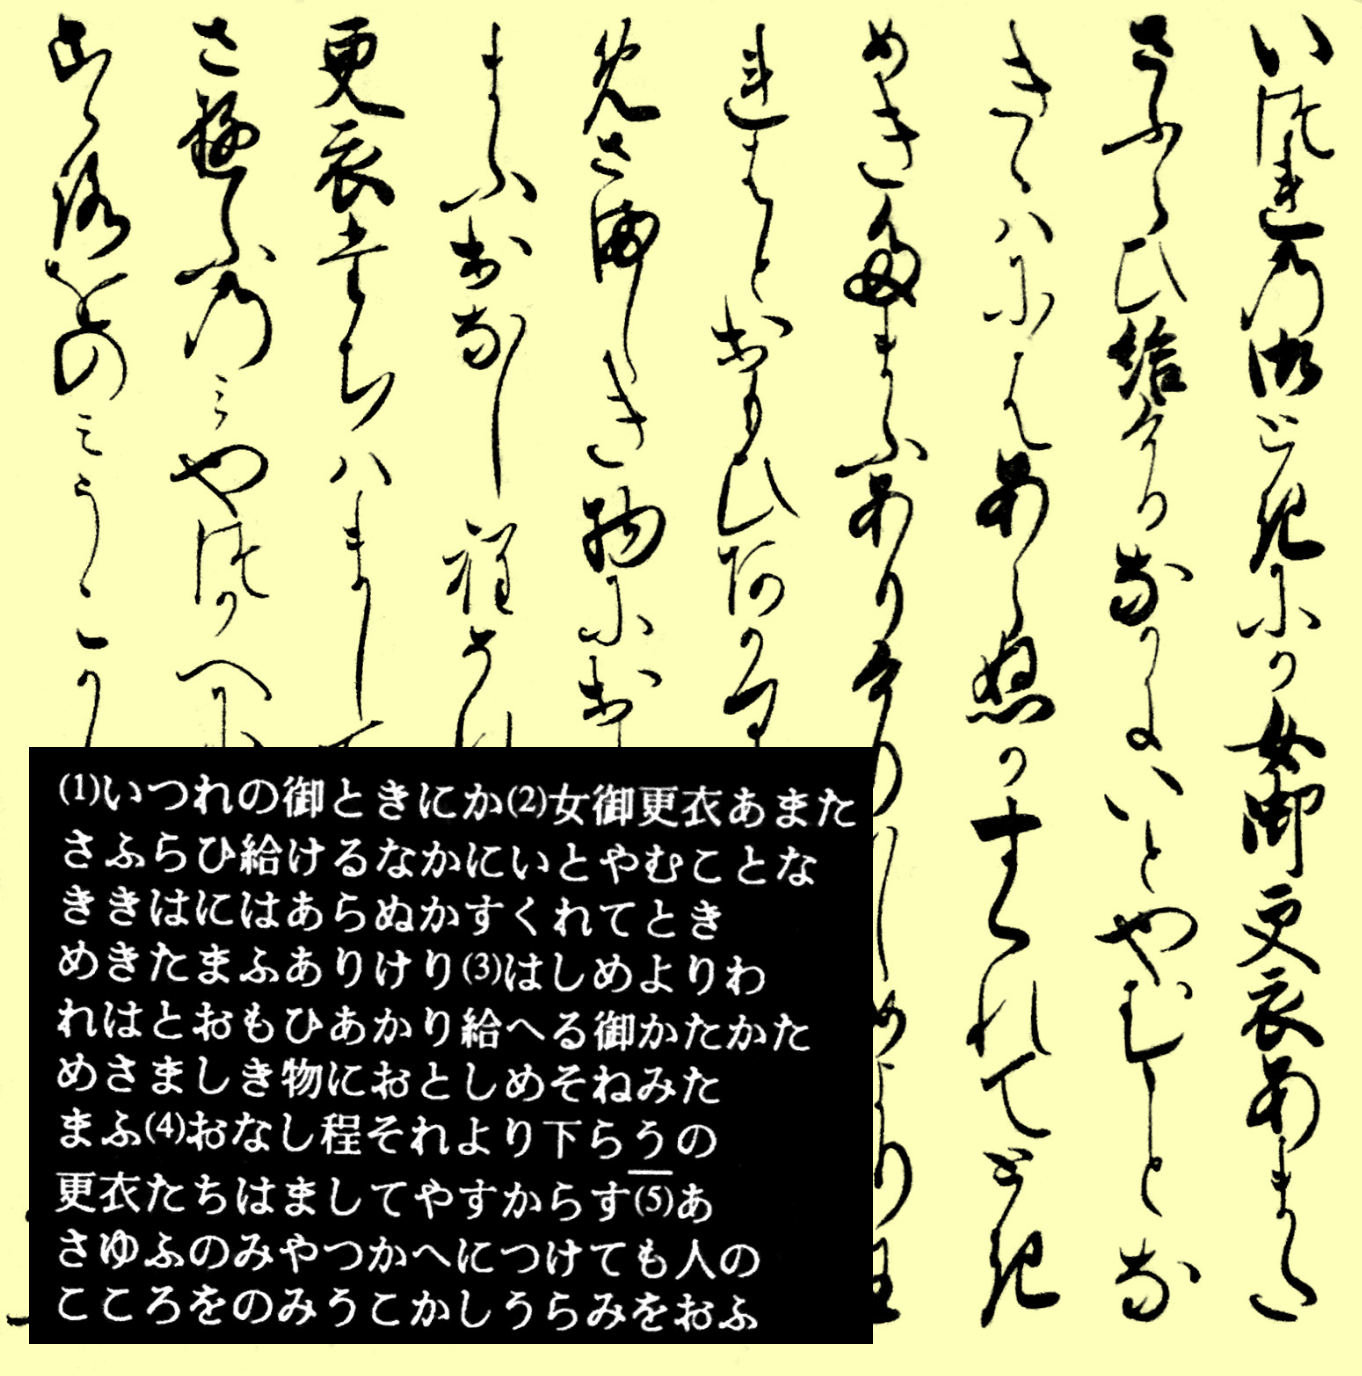
\includegraphics[width=0.55\textwidth]{\GRAPHPATH/genji3}\\
  {\tiny (\citealt{Rickmeyer1991}; 源氏物語:きりつぼ, ca. 1000 u.\,Zr., Manuskript ca.\ 1200 u.\,Zr.}
\end{frame}

\begin{frame}
  {Wie selbstverständlich ist unsere Schreibung?}
  \pause
  \centering
  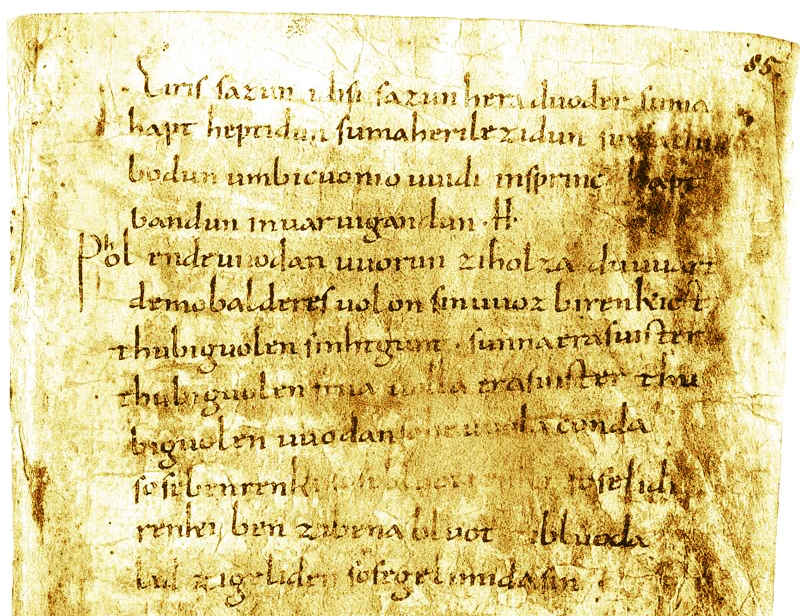
\includegraphics[width=0.8\textwidth]{\GRAPHPATH/merseburg}\\[0.5\baselineskip]
  {\tiny 1.~und 2.~Merseburger Zauberspruch, 9.~Jh.\ u.\,Zr., Cod.\ 136, Folio 85r, Domstiftsbibliothek Merseburg (Wikimedia)\\[-1\baselineskip]
    Hintergründe und generelle Einführung in historische Graphematik in \citet{Elmentaler2018}.}
\end{frame}

\begin{frame}
  {Spatien}
  \pause
  \begin{itemize}[<+->]
    \item im Ahd.\ häufig Reste von Scriptio continua
    \item syntaktische Wörter nicht immer getrennt
    \item \alert{Spatienschreibung}: Trennung syntaktischer Wörter
  \end{itemize}
  \pause
  \Halbzeile
  \begin{exe}
    \ex
    \begin{xlist}
      \ex[*]{Vanessa \rot{istgeritten}.}
      \pause
      \ex[*]{Vanessa reitet \rot{indenwald}.}
    \end{xlist}
    \pause
    \Halbzeile
    \ex
    \begin{xlist}
      \ex[*]{Vanessa hat \rot{Gelegen heit}, die \rot{Schreib ung} von Wörtern und Sätzen \rot{gründ lich} zu \rot{unter suchen}.}
      \pause
      \ex[*]{Oma \rot{koch t} der \rot{ausgekühlt en} Vanessa \rot{ein en heiß en} Tee.}
    \end{xlist}
  \end{exe}
  \pause
  \begin{itemize}[<+->]
    \item Eislaufen, Bergsteigen, Mutmachen, Teetrinken (?)
    \item weichklopfen, schlechtreden (?)
    \item nichtöffentlich, nichtprivat (?)
    \item zulasten (?)
  \end{itemize}
\end{frame}

\section[PUMS vs.\ PAMS]{Positionsunabhängige Majuskelschreibung}

\begin{frame}
  {Majuskelschreibungen}
  \pause
  \begin{itemize}[<+->]
    \item \alert{positionsabhängig}: Satzanfang (Syntax)
      \Halbzeile
    \item \alert{positionsunabhängig}: Substantive (Morphologie\slash Lexik)
    \item Positionsunabhängige Majuskelschreibung (PUMS)
      \Halbzeile
    \item Bredel: "`NP-Kopf-Großschreibung"' (= positions\rot{abhängig}, PAMS)
      \begin{itemize}[<+->]
        \item nein, weil auch in Listen, Überschriften usw.
        \item außerdem: dann Annahme SubstP als verschieden von PronP!\\
          \grau{Oder werden Pronomina als NP-Köpfe großgeschrieben?}
        \item jede Rettungsargumentation des PAMS-Ansatzes wird zirkulär 
        \item \ldots oder \alert{motiviert} die PUMS statt sie zu beschreiben
        \item \grau{Siehe Schäfer \& Sayatz (in Vorb.).}
      \end{itemize}
  \end{itemize}
\end{frame}


\begin{frame}
  {Propblemfälle für PUMS}
  \pause
  \begin{exe}
    \ex
    \begin{xlist}
      \ex{An der Nacht auf dem Land schätze ich vor allem \alert{das Dunkle}.}
      \pause
      \ex{Alle Pferde müssen geputzt werden. Vanessa putzt \alert{das schwarze}.}
      \pause
      \ex{Vanessa trägt in der Oper \alert{das Schwarze}.}
    \end{xlist}
    \Viertelzeile
    \pause
    \ex
    \begin{xlist}
      \ex[ ]{im \alert{übrigen}}
      \pause
      \ex[*]{im literarischen \rot{Übrigen}}
      \pause
      \ex[*]{Im \rot{Übrigen}\slash In dem \rot{Übrigen}, von dem wir gestern schon gesprochen haben, ist dieses Buch langweilig.}
    \end{xlist}
    \pause
    \Viertelzeile
    \ex
    \begin{xlist}
      \ex[*]{Edgar gab dem Kunden fachmännisches Recht.}
      \pause
      \ex[*]{Edgar setzte den Cadillac in einwandfreien Stand.}
    \end{xlist}
  \end{exe}
  \pause
  \begin{itemize}[<+->]
    \item Konversion
    \item Ellipse
    \item Ellipse plus Lexikalisierung
  \end{itemize}
\end{frame}

\section{Univerbierung von N+V}

\newcommand{\exhl}[1]{\alert{#1}}

\begin{frame}
  {Grenzfall für Spatien und PUMS}
  Was würden Sie machen?\\
  \Zeile
  \begin{exe}
  \ex\label{ex:introexamples1}
  \begin{xlist}
    \ex Yael weiß, dass Remy \exhl{Rad} \exhl{fährt}.
    \ex Yael weiß, dass Remy \exhl{radfährt}.
  \end{xlist}
  \Zeile
  \ex
  \begin{xlist}
    \ex Yael weiß, dass Remy \exhl{Eis} \exhl{läuft}.
    \ex Yael weiß, dass Remy \exhl{eisläuft}.
  \end{xlist}
\end{exe}
\end{frame}

\begin{frame}
  {Syntaktische Kontexte | Getrenntschreibung}
  Was kann man auseinander schreiben?\\
  \Zeile
  \begin{exe}
  \ex
  \begin{xlist}
    \ex[ ]{Remy \exhl{fährt} gerade \exhl{Rad}.}
    \ex[ ]{Remy ist gestern \exhl{Rad} \exhl{gefahren}.}
    \Zeile
    \ex[ ]{Remy hat keine Lust, \exhl{Rad} \exhl{zu} \exhl{fahren}.}
    \ex[ ]{Yael weiß, dass Remy \exhl{Rad} \exhl{fährt}.}
    \ex[ ]{Remy will \exhl{Rad} \exhl{fahren}.}
    \Zeile
    \ex[ ]{Remy ist am \exhl{Rad} \exhl{fahren}.}
    \Zeile
    \ex[ ]{Remy singt beim \exhl{Rad} \exhl{fahren}.}
    \ex[*]{Remy lobt das \exhl{Rad} \exhl{fahren}.}
    \end{xlist}
  \end{exe}
\end{frame}

\begin{frame}
  {Syntaktische Kontexte | Zusammenschreibung}
  \begin{exe}
  \ex
  \begin{xlist}
    \setcounter{xnumii}{1}
    \ex[ ]{Remy ist gestern \exhl{radgefahren}.}
    \ex[ ]{Remy hat keine Lust, \exhl{radzufahren}.}
    \ex[ ]{Yael weiß, dass Remy \exhl{radfährt}.}
    \ex[ ]{Remy will \exhl{radfahren}.}
    \ex[ ]{Remy ist am \exhl{Radfahren\slash radfahren}.}
    \ex[ ]{Remy singt beim \exhl{Radfahren\slash radfahren}.}
    \ex[ ]{Remy lobt das \exhl{Radfahren}.}
  \end{xlist}
\end{exe}
\end{frame}


\begin{frame}
  {Mögliche Einflussfaktoren}
  \begin{itemize}[<+->]
    \item (morpho-)syntaktischer \alert{Kontext}
      \begin{itemize}[<+->]
        \item Infinitiv
        \item Partizip
        \item \textit{am}-Progressiv
        \item NP (in Präposition)
      \end{itemize}
      \Zeile
    \item \alert{semantische Relation} zwischen N und V
      \begin{itemize}[<+->]
        \item Argument
        \item oblique
        \item unbestimmbar
      \end{itemize}
      \Zeile
    \item individuelle \alert{Lexikalisierungstendenz}\\
      \grau{stärkere Bildung eines neuen komplexen semantischen Konzepts}
  \end{itemize}
\end{frame}

\begin{frame}
  {Schäfer \& Sayatz (eingereicht)}
  \centering 
  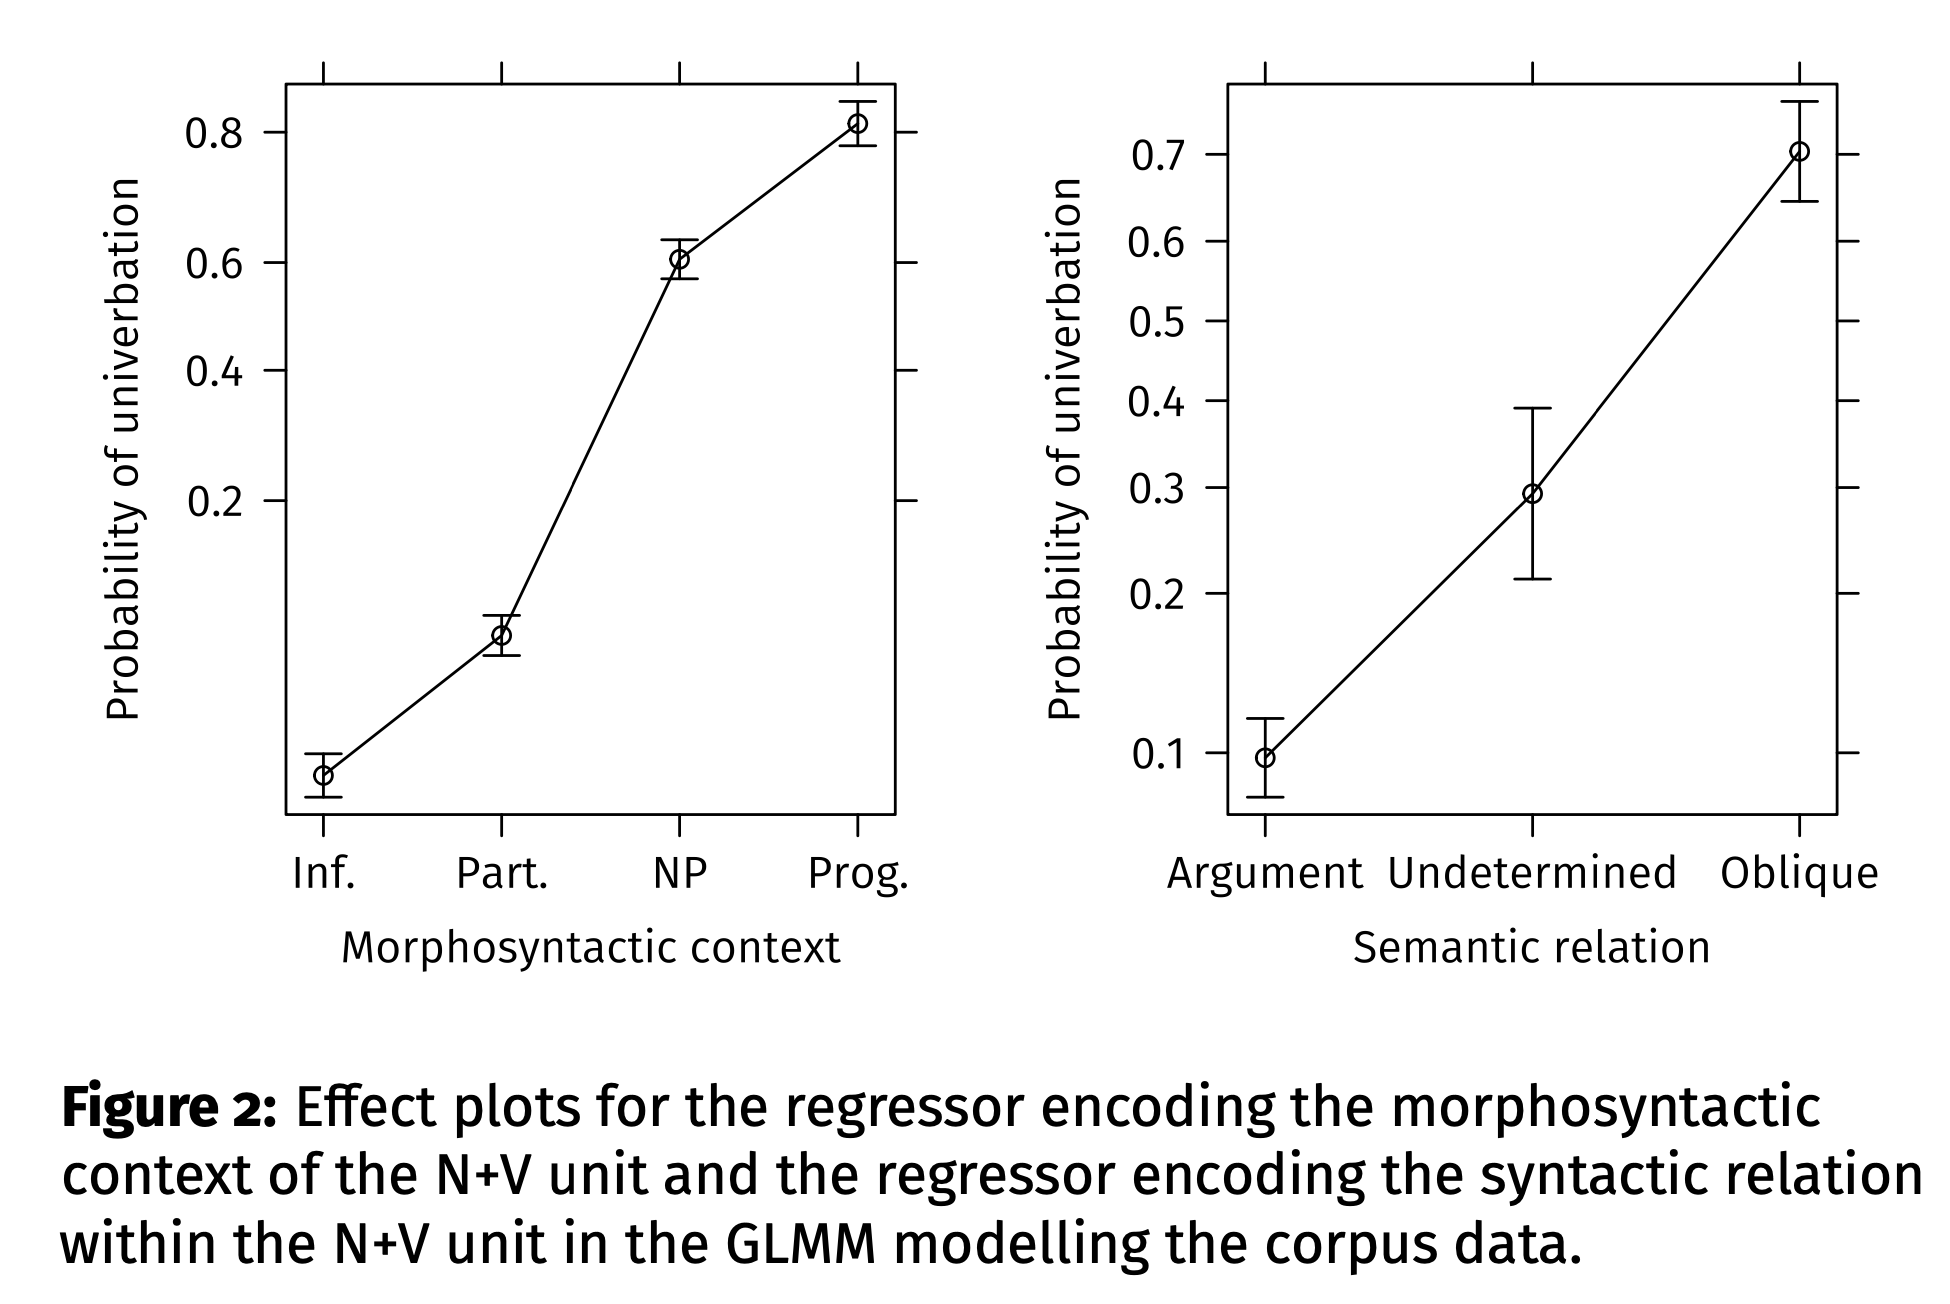
\includegraphics[width=0.7\textwidth]{\GRAPHPATH/nv2}
\end{frame}

\begin{frame}
  {Schäfer \& Sayatz (eingereicht)}
  \centering 
  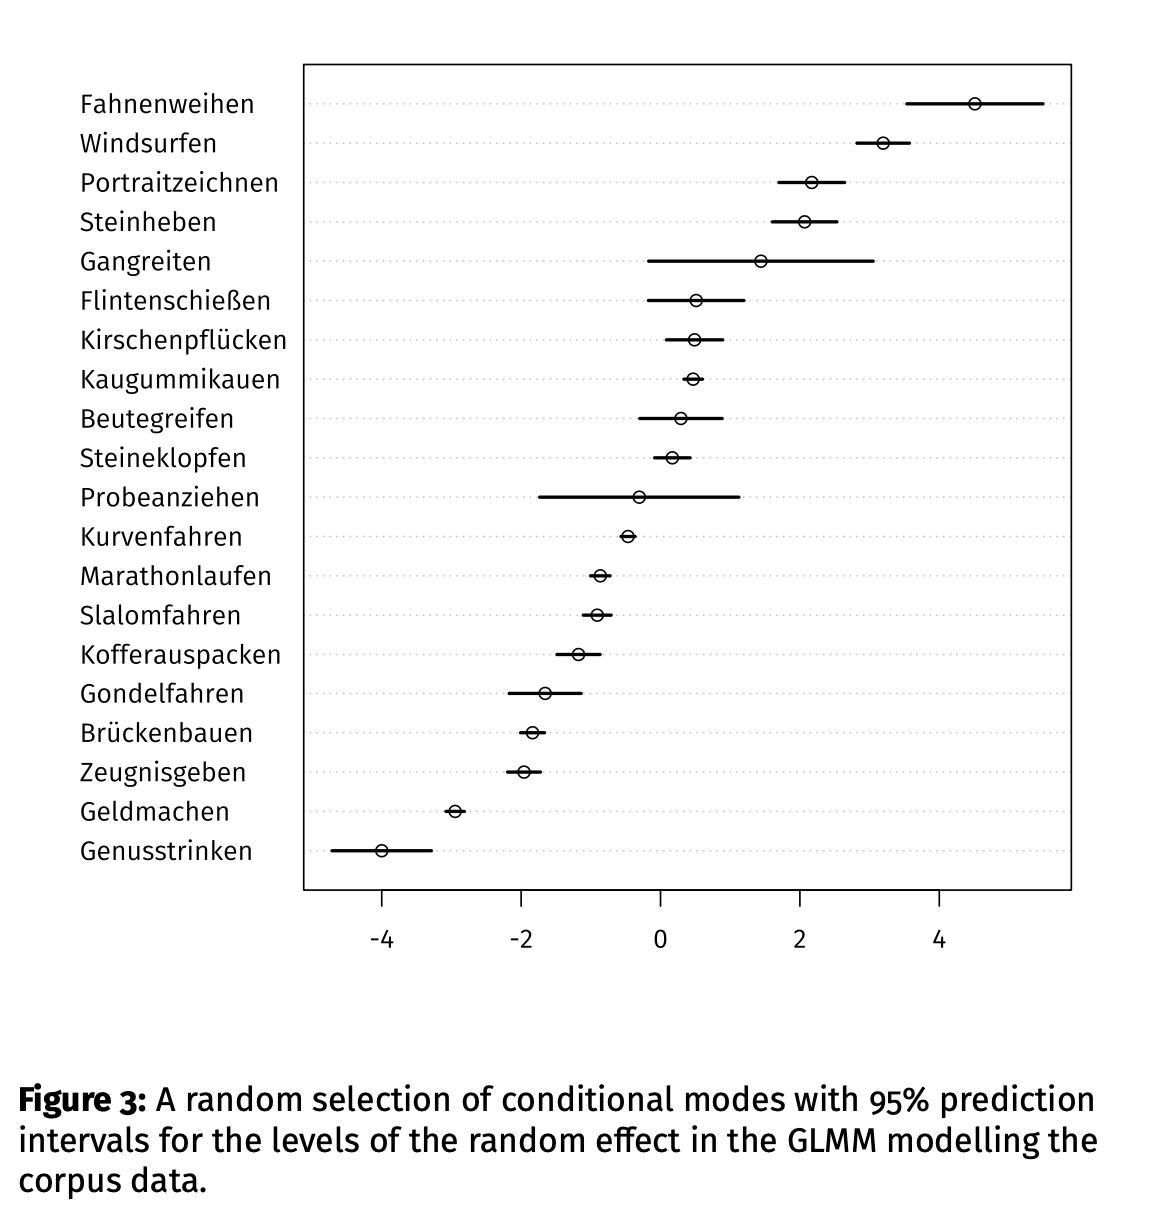
\includegraphics[width=0.7\textwidth]{\GRAPHPATH/nv3}
\end{frame}

\begin{frame}
  {Schäfer \& Sayatz (eingereicht)}
  \centering 
  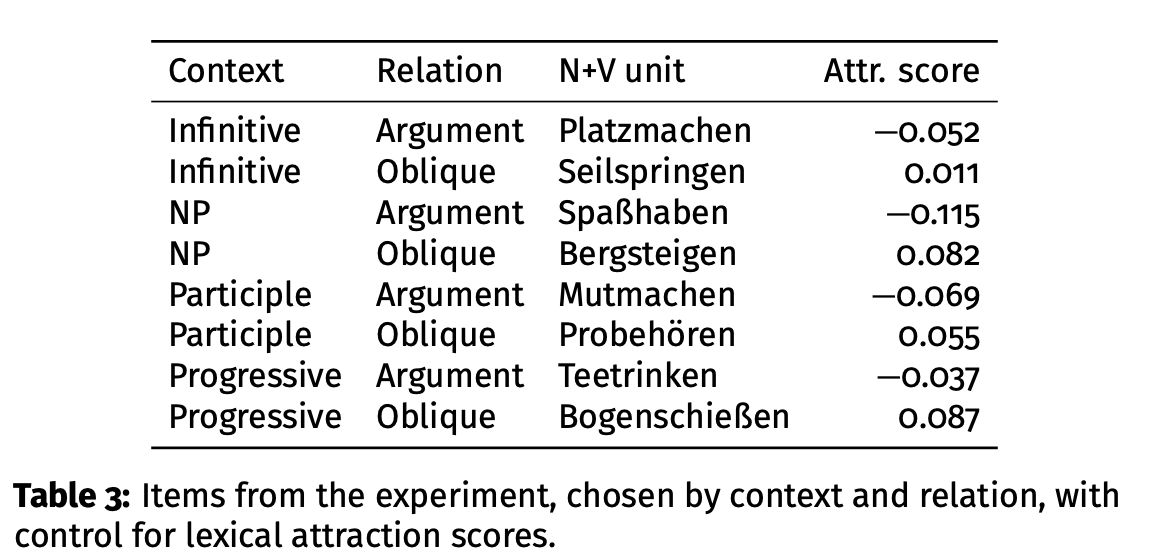
\includegraphics[width=0.7\textwidth]{\GRAPHPATH/nv4}
\end{frame}

\begin{frame}
  {Schäfer \& Sayatz (eingereicht)}
  \centering 
  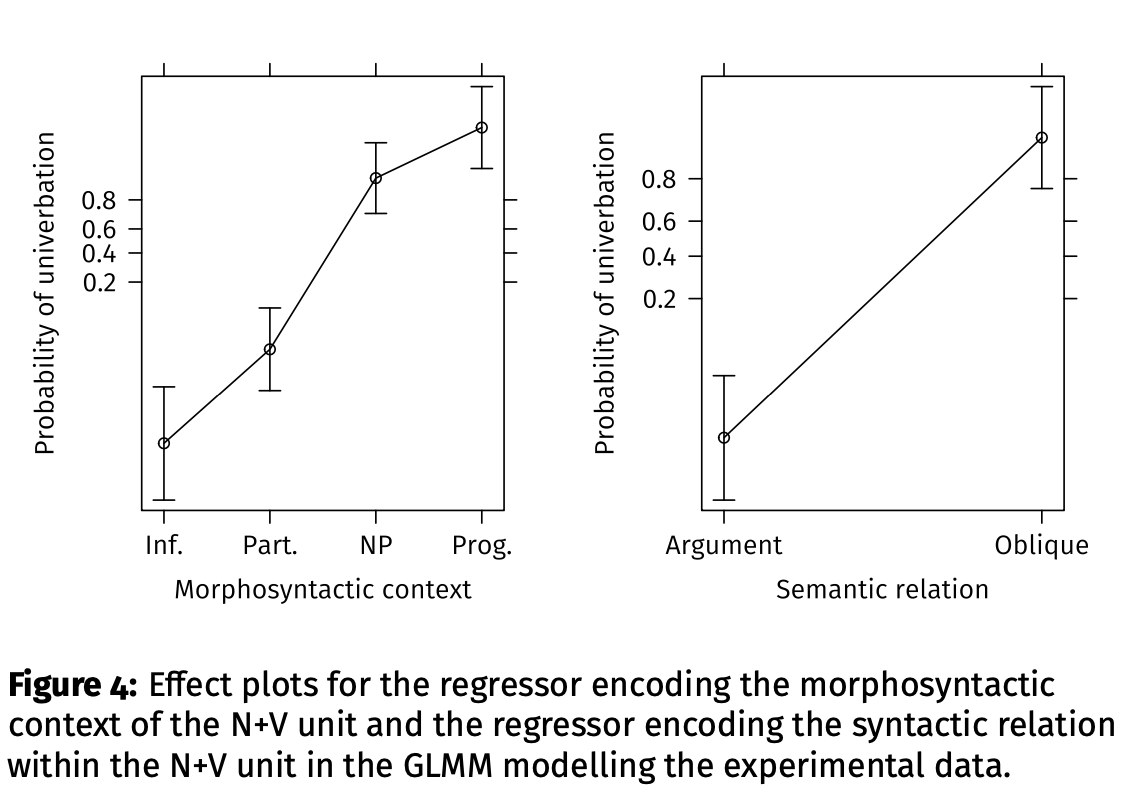
\includegraphics[width=0.7\textwidth]{\GRAPHPATH/nv5}
\end{frame}

\begin{frame}
  {Schäfer \& Sayatz (eingereicht)}
  \centering 
  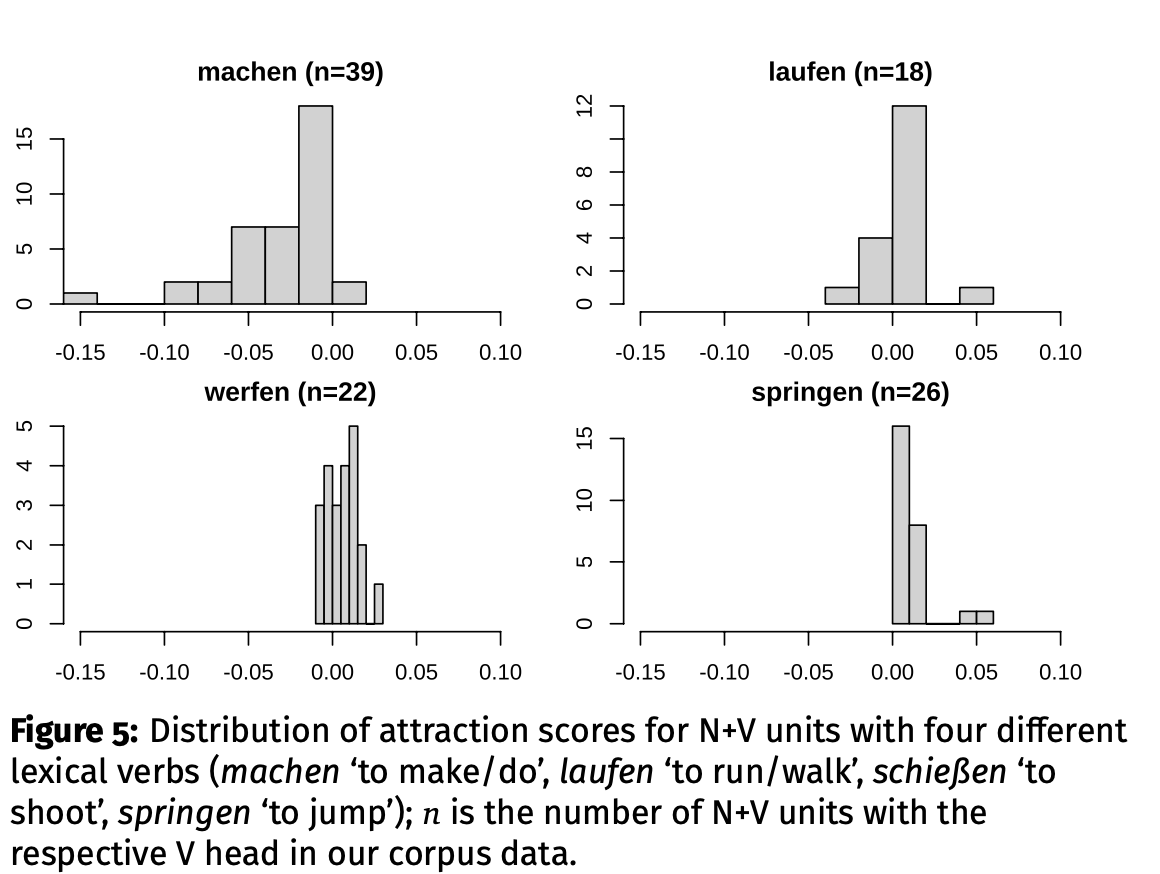
\includegraphics[width=0.7\textwidth]{\GRAPHPATH/nv6}
\end{frame}

\begin{frame}
  {Grundsätzliche theroretische Erkenntnis}
  Gebrauchsbasierte Graphematik\\
  \Zeile
  \begin{itemize}[<+->]
    \item Lernen von Generalisierungen über Ähnlichkeiten
    \item konfligierende Beschränkungen\slash Einflussfaktoren
    \item nicht immer harte Trennung | \alert{probabilistische Grammatik}
      \Zeile
    \item arbiträre Normierung
    \item klarer Fall für permissive Normierung
  \end{itemize}
\end{frame}


\ifdefined\TITLE
  \section{Nächste Woche | Überblick}

  \begin{frame}
    {Der ungefähre Semesterplan}
    \begin{enumerate}[<+->]
      \item Graphematik und Schreibprinzipien
      \item Wiederholung -- Phonetik
      \item Wiederholung -- Phonologie
      \item Phonographisches Schreibprinzip -- Konsonanten
      \item Phonographisches Schreibprinzip -- Vokale
      \item Silben und Dehnungsschreibungen
      \item Eszett, Dehnung und Konstanz
      \item Spatien und Majuskeln
      \item \alert{Komma}
      \item Punkt und sonstige Interpunktion
    \end{enumerate}
  \end{frame}
\fi

